\chapter{Electric currents}

\section{Charge transport and current density}

Electric currents are caused by the motion of charge carriers. The
electric current in a wire is a measure of the amount of charge passing
any point of the wire per unit time. In the units we have been
using, current would be expressed in esu per second. The practical
unit is the ampere, which amounts to one coulomb of charge per
second. A current of one ampere is the same as a current of
$3 \times 10^9\ \esu/\sunit$, which is equivalent to $6.2 \times 10^{13}$ electrons per
second. Of course, it is always the net charge transport that counts,
with due regard to sign. The motion of a neutral body could be said
to involve the transport of a tremendous amount of charge (some
$10^5$ coulombs per gram of matter!), but there is no current because
exactly the same number of positive and of negative elementary
particles are moving with exactly the same average velocity.

A more general kind of current, or charge transport, involves
charge carriers moving around in a three-dimensional volume. To
describe this we need the concept of \intro{current density}. We have to
consider average quantities, for charge carriers are discrete particles.
We must suppose, as we did in defining the charge density p, that
our scale of distances is such that any small region we wish to average
over contains very many particles of any class we are concerned
with.

Consider first a special situation in which there are $n$ particles
per cubic centimeter, on the average, all moving with the same vector
velocity $\vc{u}$ and carrying the same charge $q$. Imagine a small frame
of area $\vc{a}$ fixed in some orientation, as in Fig. 4.1a. How many particles
pass through the frame in a time interval $\Delta t$? If $\Delta t$ begins the
instant shown m Fig. 4.1a and b, the particles destined to pass
through the frame in the next $\Delta t$ sec will be just those now located
within the oblique prism in Fig. 4.11). This prism has the frame area
of its base and an edge length $u \Delta t$, which is the distance any particle
will travel in a time $\Delta t$. Particles outside this prism will either miss
the window or fail to reach it. The volume of the prism is the product
\emph{base} $\times$ \emph{altitude}, or $au \Delta t \cos \theta$, which can be written
$\vc{a}\cdot\vc{u} \Delta t$. On
the average, the number of particles found in such a volume will be
$n\vc{a}\cdot\vc{u} \Delta t$. Hence the average rate at which charge is passing through
% p. 111
the frame, that is, the current through the frame which we shall call
$I(a)$, is
\begin{equation}
  I(a) = \frac{q(n\vc{a}\cdot\vc{u} \Delta t)}{\Delta t} = nq\:\vc{a}\cdot\vc{u}
\end{equation}

Suppose we had many classes of particles in the swarm, differing
in charge, in velocity vector, or in both. Each would make its own
contribution to the current through $\vc{a}$. Denoting each kind by a subscript
$k$, the $k$th class has charge $q_k$ on each particle, moves with
velocity vector $\vc{u}_k$, and is present with an average population density
of $n_k$ such particles per cubic centimeter, and we could state this in a
formal way:
\begin{equation}
  I(a) = n_1q_1 \vc{a}\cdot\vc{u}_1+n_2q_2 \vc{a}\cdot\vc{u}_2+\ldots
         = \vc{a}\cdot\sum_k n_kq_k\vc{u}_k
\end{equation}
The vector quantity in Eq. 2 that multiplies $\vc{a}$ we call the current
density $\vc{J}$. $\vc{J}$ could be expressed in units of esu per second per square
centimeter. If we are using practical units with the coulomb as the
unit of charge, the current density will be expressed in amperes per
square centimeter.
\begin{equation}
  \vc{J} = n_kq_k\vc{u}_k
\end{equation}

Let's look at the contribution to the current density from one
variety of charge carriers, electrons say, which may be present with
many different velocities. In a conductor, the electrons will have
an almost random distribution of velocities, varying widely in direction
and magnitude. Let $N_e$ be the total number of electrons per
unit volume, of all velocities. We can divide the electrons into many
groups, each of which contains electrons with nearly the same speed
and direction. The \emph{average velocity} of all the electrons, like any
average, would then be calculated by summing over the groups,
weighting each velocity by the number in the group, and dividing by
the total number. That is,
\begin{equation}
  \bar{\vc{u}} = \frac{1}{N_e} \sum_k n_k\vc{u}_k
\end{equation}
We use the bar over the top of $\bar{\vc{u}}$ to mean the average over a distribution.
Comparing Eq. 4 with Eq. 3, we see that the contribution
of the electrons to the current density can be written simply in terms
of the average electron velocity. Remembering that for the electron
% p. 112
$q=-e$, and using subscript $e$ to show that all quantities refer to
this one type of charge carrier, we can write
\begin{equation}
  \vc{J}_e = -eN_e \bar{\vc{u}}_e
\end{equation}

This may seem rather obvious, but we have gone through it step
by step to make clear that the current through the frame depends
only on the \emph{average} velocity of the carriers, which often is only a tiny
fraction, in magnitude, of their random speeds. Don't forget that
Eq. 4 describes a \emph{vector} average; it will be zero for a distribution of
velocities in which all directions are equally likely, whatever the
speeds may be.

\section{Stationary currents}
The current carried by a long conductor like a wire is, of course,
just the integral of the current density $\vc{J}$ over the cross section of the
wire. Indeed, the current $I$ flowing through any surface $S$ is just the
surface integral
\begin{equation}
  I = \int_S \vc{J}\cdot\der\vc{a}
\end{equation}
$I$ is the ``flux'' associated with the vector $\vc{J}$, and in this case the name
is apt.

We speak of a steady or stationary current system when the current
density vector $\vc{J}$ remains constant in time everywhere. Steady
currents have to obey the law of charge conservation. Consider
some region of space completely enclosed by the balloonlike surface
$S$. The surface integral of $\vc{J}$ over all of $S$ gives the rate at which
charge is leaving the volume enclosed. It will be positive if positive
charge carriers are moving outward or negative charge carriers are
moving inward, and so on. Were this to go on indefinitely, the volume
would sooner or later run out of charge---unless some new
charge were created. But charge creation is just what can't happen.
Therefore, for a truly time-independent current distribution, the
surface integral of $\vc{J}$ over any closed surface must be zero. This is
completely equivalent to the statement that, at every point in space:
\begin{equation}
  \div\vc{J}=0 \qquad \text{(time-independent charge distribution)}
\end{equation}
To appreciate the equivalence, recall Gauss's theorem and our fundamental
definition of divergence in terms of the surface integral
over a small surface enclosing the location in question.

% p. 113
We can make a more general statement than Eq. 7. Suppose the
current is not steady, $\vc{J}$ being a function of $t$ as well as of $x$, $y$, and $z$.
Then since $\int_S \vc{J}\cdot\der\vc{a}$ is the instantaneous rate at which charge is
\emph{leaving} the enclosed volume, while $\int_V\rho\der v$ is the total charge inside
the volume at any instant, we have
\begin{equation}
  \int_S \vc{J}\cdot\der\vc{a} = -\frac{\der}{\der t} \int_V\:\rho\der v
\end{equation}
Letting the volume in question shrink down around any point
$(x,y,z)$, the relation expressed in Eq. 8 becomes:\footnote{If
the step between Eqs. 8 and 9 is not obvious, look back at our fundamental definition
of divergence in Chap. 2. As the volume shrinks, we can eventually take $\rho$ outside
the volume integral on the right. The volume integral is to be carried out at one instant
of time. Its time derivative thus depends on the difference between the volume integral
at $t$ and at $t + \der t$. The only difference is due to the change of $\rho$ there, since the boundary
of the volume remains in the same place.}
\begin{equation}
  \div\vc{J}=-\frac{\partial\rho}{\partial t} \qquad \text{(time-dependent charge distribution)}
\end{equation}
The time derivative of the charge density $\rho$ is written as a partial
derivative since $\rho$ will usually be a function of spatial coordinates as
well as time. Equations 8 and 9 express the conservation of charge:
No charge can flow away from a place without diminishing the
amount of charge that is there.

An instructive example of a stationary current distribution occurs
in the plane diode, a two-electrode vacuum tube. One electrode, the
cathode, is coated with a material that emits electrons copiously
when heated. The other electrode, the anode, is simply a metal plate.
By means of a battery the anode is maintained at a positive potential
with respect to the cathode. Electrons emerge from this hot
cathode with very low velocities, but are then accelerated toward the
positive anode by the electric field between cathode and anode. In
the space between the cathode and anode the electric current consists
of these moving electrons. The circuit is completed by the flow
of electrons in external wires, possibly by the movement of ions in
a battery, and so on, with which we are not here concerned. In this
diode, the local density of charge in any region, $\rho$, is simply $-ne$
where $n$ is the local density of electrons, in $\zu{electrons}/\cmunit^3$. The local
current density $\vc{J}$ is of course $\rho \vc{v}$ where $\vc{v}$ is the velocity of electrons
in that region. In the plane-parallel diode we may assume $\vc{J}$ has no
$y$ or $z$ components (Fig. 4.2). If conditions are steady, it follows
% p. 114
then that $J_x$ must be independent of $x$, for if $\div\vc{J} = 0$ as Eq. 7 says,
$(\partial J_x/\partial x)$ must be zero if $J_y = J_z = 0$. This is belaboring the obvious;
if we have a steady stream of electrons moving in the $x$ direction
only, the same number per second have to cross any intermediate
plane between cathode and anode. We conclude that $\rho v$ is constant.
But observe that $v$ is not constant; it varies with $x$ because the electrons
are accelerated by the field. Hence $\rho$ is not constant either.
Instead, the negative charge density is high near the cathode, low
near the anode, just as the density of cars on an expressway is high
near a trafiic slowdown, low where traffic is moving at high speed.
The current in a diode may be limited by an interesting effect: the
inffuence of the negative charge density (the ``space charge'') on the
electric field, hence on the acceleration and velocity of the electrons,
hence---completing the circle---on the charge density itself. 
Problem 4.25 explores the behavior of the ``space-charge-lirnited'' diode
and indicates how you can derive the curious voltage-current relation
which governs it. The relation is important in electronics not only
in the design and use of diodes but also in the design of electron guns
for cathode-ray tubes and the like.

\section{Electrical conductivity and Ohm's law}

There are many ways of causing charge to move, including what
we might call ``bodily transport'' of the charge carriers. In the
Van de Graaff electrostatic generator (see Prob. 4.3) an insulating
belt is given a surface charge, which it conveys to another electrode
for removal, much as an escalator conveys people. That constitutes
a perfectly good current. In the atmosphere, charged water droplets
falling because of their weight form a component of the electrical
current system of the earth. In this section we shall be interested in
a more common agent of charge transport, the force exerted on a
charge carrier by an electric field. An electric field tends to make
charge carriers move and thus tends to cause an electric current.
Whether or not it does so depends on the physical nature of the system
within which the field acts, the \emph{medium}.

One of the earliest experimental discoveries about electric currents
in matter is summarized in Ohm's law:
\begin{equation}
  I = \frac{V}{R}
\end{equation}
% p. 115
The current $I$ flowing through a wire is proportional to $V$, the difference
in potential between its ends. We have used $\pot$ heretofore as
the symbol for electric potential, and $(\pot_1-\pot_2)$ or $\pot_{12}$ for the difference
of potential. In this section we shall use the symbol $V$, which
is more common in the elementary physics of electric circuits, and
comes, of course, from ``volts'' or ``voltage.'' (We had avoided $V$
merely because it suggests so many different things: Volume, velocity,
voltage.)

For a given piece of wire maintained at the same temperature, the
resistance $R$, the constant of proportionality in Eq. 10, does not depend
on the amount of current flowing. The resistance does depend
in an obvious way on the length and cross section of the wire, being
proportional to the length $L$ and inversely proportional to the area
of cross section $A$. Of course it also depends on the material of
which the conductor is made and all of this is expressed in the simple
formula:
\begin{equation}
  R = \rho \frac{L}{A}
\end{equation}
The factor $\rho$ is called the volume resistivity of the substance. Usually
resistance is measured in ohms, $\Omega$, which goes with amperes for current
and with volts for potential difference in Ohm's law. The corresponding
unit of resistivity is the ohm-centimeter, $\Omega\unitdot\cmunit$, if lengths are measured
in centimeters, and this is the unit which is commonly given in tables.

The electrical engineer is interested in Eqs. 10 and 11 chieffy for
calculating the resistance of parts of electrical circuits, and the
voltage-current relations in those circuits. The physicist---except
when he is designing electrical apparatus---sees these equations as
reflecting a most remarkable and general property of matter, which
it is his task to understand. The fundamental fact which the 
equations, taken together, reflect, is this: In solid homogeneous materials
the current density at any point is proportional to the electric field
and the constant of proportionality depends only on the substance---
not, for instance, on the shape of the conductor. That is,
\begin{equation}
  \vc{J}=\sigma\vc{E}
\end{equation}
where $\sigma$ is a constant characteristic of the substance.

In the interior of most conductors, three perpendicular directions
are physically equivalent. For instance, in copper the atoms are
arranged on a cubic (face-centered cubic) lattice. But even when
its atomic arrangement is not cubical, a piece of metal is usually
% p. 116
composed of many small crystals randomly oriented, which makes
all directions equivalent in any large-scale average. In all such 
substances, there being no preferred direction, $\vc{J}$ will have the same
direction as $\vc{E}$, and the constant $\sigma$ is simply a 
sca1ar.\footnote{ln general, a linear relation between two vectors involves a tensor. We'1l meet an
important example of a tensor in Chap. 9. There are a few substances in which the
conductivity is quite different in different directions and has to be treated as a tensor,
but we needn't worry about them.} 
We call it the
electrical \intro{conductivity} of the material. The conductivity $\sigma$ is just the
reciprocal of the resistivity 
$\rho$.\footnote{The Greek letters $\rho$ and $\sigma$ are the symbols usually adopted for resistivity and con-
ductivity, in spite of their equally common usage for volume charge density and surface
charge density. There just aren't enough letters to go round.} Figure 4.3 summarizes these simple
relations, and shows how Eqs. 10 and 11 are implied by Eq. 12.

% p. 117

A word about units and dimensions. The common unit for conductivity
is derived from the practical unit of resistance, the ohm. As
you well know, the ohm is one volt per ampere. Conductivity is the
ratio $\frac{\text{current density}}{\text{field strength}}$
which in practical units would be
$\frac{\zu{amperes}/\cmunit^2}{\zu{volts}/\cmunit}$
or $(\ohmunit\unitdot\cmunit)^{-1}$, often read as ``reciprocal ohm-centimeter.'' More
often, the reciprocal of the conductivity, called the \intro{resistivity}, is given.
The practical unit is the ohm-centimeter, and the usual symbol is $\rho$.
The resistivity of a good conductor at room temperature is typically
a few millionths of an ohm-centimeter. Thus pure copper has a
resistivity at room temperature of $1.7 \times 10^{-6}\ \ohmunit\unitdot\cmunit$, or a conductivity
of $5.8\times 10^5\ \ohmunit\unitdot\cmunit^{-1}$.

In the CGS electrostatic system there is no special name for the
unit of conductivity or resistivity, but since that system of units is
built on the centimeter, gram, and second, and nothing else, the unit
must be some combination of these. What, for instance, are the
dimensions of resistivity?
\begin{equation}
  \text{Resistivity} = \frac{\text{field strength}}{\text{current density}}
    = \left. 
        \left(\frac{\text{charge}}{\cmunit^2}\right)
      \middle/ 
        \left(\frac{\text{charge}/\sunit}{\cmunit^2}\right)
      \right.
\end{equation}
which reduces simply to seconds. Resistivity has the dimensions of
time, and the appropriate name for the unit would be the \emph{second!}
In these units the resistivity of copper is $10^{-17}$ s, that of glass at
room temperature of the order of $10^3$ s. We shall find later that
this curious association of a time with a \emph{material} has a reasonable
physical interpretation.

\section{A model for electrical conduction}

Equation 12 is merely a description of the observed behavior of
most familiar substances over a certain range of conditions. We
cannot derive it from the fundamental laws of the electric field. To
understand its significance we have to understand the processes that
go on in a particular substance when an electric field is applied, and
these may be very different in different kinds of matter. What is
truly remarkable about Ohm's law is the variety of substances and
the wide range of field strengths over which it is quite accurately
obeyed. (It does fail, indeed it \emph{must} fail, in some circumstances, and
we shall discover some reasons why.) We shall try now to describe
% p. 118
in detail the process of electrical conduction in one model system.
It will be reasonably typical of a wide class of electrical conductors,
but not of all.

We need charge carriers, so let us imagine a medium consisting of
positive and negative charge carriers in equal number, say $N$ of each
kind per cubic centimeter. The positive carriers are ions of mass $M_+$
each, carrying charge $e$, while the negative carriers are negative ions
of mass $M_-$ each, with charge $-e$. The current density $\vc{J}$ will be
determined by the average velocities of these carriers.

A uniform electric field \vc{E}, constant in time, is applied to this system,
exerting a force on every charge carrier. This is the first occasion,
in this volume, on which we have considered the force on a
moving charge in an electric field. We shall treat the question carefully
in Chap. 6. The fact is---and it was already used in Vol. I---that
the force is the same as if the charge carrier were at rest. That is,
each carrier of charge $q$, regardless of its motion, experiences the
constant force $q\vc{E}$.

At this point let us pause to marvel that Ohm's law is ever obeyed!
A constant force on a free charge carrier ought to produce a constant
acceleration. But constant current density is associated with constant
\emph{velocity}, not constant acceleration. If our system really does
obey Ohm's law, it must be because average \emph{velocity} is proportional
to {force}, for our carriers. This warns us that the charge carriers cannot
be moving freely; there must be something which opposes the
motion that the electric field causes.

We do not have to look far to find a source of frictional hindrance
---it arises from the collisions the charge carriers experience as they
move among one another and among any other particles that may
inhabit the medium.

Just how this works out will depend somewhat on the details of
our model. Let us be rather specific and think of a gas consisting of
neutral atoms, positive ions, and negative ions at something like normal
gas density, roughly $10^{19}$ $\zu{atoms}/\cmunit^3$ (Fig. 4.4). Suppose there
is a preponderance of neutral atoms, with positive and negative ions
here and there among them. The distance between particles,
whether neutral or charged, is much larger than the atomic or ionic
radii so that an ion spends most of its time \emph{not} involved in a close
collision.

In the absence of an electric field the atoms and ions will be moving
about in random directions, with speeds that are determined by
the temperature. The kinetic theory of gases can give us the relation,
% p. 119
if we should need it, between the temperature and the average
kinetic energy of a particle. If we could look in at a particular ion
at a particular instant, say $t = 0$, we would find it moving with some
velocity $\vc{u}$. What will happen next? The ion will move in a straight
line at constant speed until, presently, it chances to come close to an
atom, close enough for short-range forces to come into play. In this
collision, the total kinetic energy and the total momentum of the two
bodies will be conserved, but the speed and direction of the ion's
ffight will be altered---perhaps only a little, perhaps drastically---to
a new velocity $\vc{u}'$. Later a new collision occurs, changing the velocity
to $\vc{u}''$, and so it goes. It can also happen that another ion some distance
away, interacting with our ion by the long-range Coulomb
force, deflects the ion's path. Long-range encounters, which can be
important between ions and ions, mostly change the velocity in
smaller random increments, but the eventual effect is the same.
The eventual effect---and this is the key to our problem---is to wipe
out any relation (either in magnitude or direction) between the
velocity $\vc{u}$ of the ion at $t = 0$ and its velocity after some interval has
elapsed. That is to say, after some time $t = \tau$ the ion's velocity vector
is as likely to be found pointing in one direction in space as in
another, regardless of the direction it had at $t = 0$. The ion has
``forgotten'' the direction in which it was originally moving. To put
it another way, if we picked 10,000 cases of ions moving horizontally
south, and followed each of them for $\tau$ seconds, their final velocity
directions would be distributed impartially over a sphere. It may
take several collisions to wipe out most of the direction memory or
only a few, depending on whether collisions involving large momentum
changes or small momentum changes are the more common,
and this depends on the nature of the interaction. An extreme case
is the collision of hard elastic spheres, which turns out to produce a
complete directional ``shuffle'' in just one collision. We need not
worry about these differences. The point is that, whatever the nature
of the collisions, there will be \emph{some} time interval $\tau$, characteristic of
a given system, such that the lapse of $\tau$ seconds leads to substantial
loss of correlation between the initial velocity direction and the final
velocity direction of an ion in that
system.\footnote{It would be possible to define $\tau$ precisely for a general system by giving a quantitative
measure of the correlation between initial and final directions. It is a statistical 
problem, like devising a measure of the correlation between the birth weights of rats and
their weights at maturity. However, we shall not need a general quantitative definition
to complete our analysis.
} This characteristic time
% p. 120
$\tau$ will depend on the ion and on the nature of its average environment;
it will certainly be shorter the more frequent the collisions,
since in our gas nothing happens to an ion between collisions.

Now we are ready to apply a uniform electric field $\vc{E}$ to the system.
It will make the description easier if we imagine the loss of direction
memory to occur completely at a single collision, as we have said it
does in the case of hard spheres. Our main conclusion will actually
be independent of this assumption. Immediately after acollision
an ion starts off in some random direction. We will denote by uc
the velocity immediately after a collision. The electric force on the
ion, Ee, imparts momentum to the ion continuously. After time $t$
it will have acquired from the field a momentum increment $\vc{E}et$,
which simply adds vectorially to its original momentum $M\vc{u}^c$. Its
momentum is now $M\vc{u}^c+\vc{E}et$. If the momentum increment is small
relative to $M\vc{u}^c$, that implies the velocity has not been affected much,
so we can expect the next collision to occur about as soon as it would
have in the absence of the electric field. In other words the average
time between collisions, which we shall denote by $\bar{t}$, is independent
of the field $\vc{E}$ if the field is not too strong.

The momentum acquired from the field is always a vector in the
same direction. But it is lost, in effect, at every collision, since the
direction of motion after a collision is random, regardless of the
direction before.

\emph{What is the average momentum of all the positive ions, at a given
instant of time?} This question is surprisingly easy to answer if we
look at it this way: At the instant in question, suppose we stop the
clock and ask each ion how long it has been since its last collision.
Suppose we get the particular answer $t_1$ from positive ion 1. Then
that ion must have momentum $E\vc{e}t_1$ in addition to the momentum
$M\vc{u}_1^c$ with which it emerged from its last collision. The average
momentum of all $N$ positive ions is therefore
\begin{equation}
  M\bar{\vc{u}}_+ = \frac{1}{N}\sum_j\left(M\vc{u}_j^c+\vc{E}et_j\right)
\end{equation}
Here $\vc{u}_j^c$ is the velocity the $j$th ion had just after its last collision.
These velocities $\vc{u}_j^c$ are quite random in direction and therefore contribute
zero to the average. The second part is simply $\vc{E}e$ times the
\emph{average of the $t_j$}, that is, times the \emph{average of the time since the last
collision}. That must be the same as the average of the time to the
% p. 121
\emph{next} collision, and both
are the same\footnote{You may think the average time between collisions would have to be equal to the
\emph{sum} of the \emph{average time since the last collision} and the \emph{average time to the next}. That
would be true if collisions occurred at absolutely regular intervals, but they don't. They
are independent random events, and for such the above statement, paradoxical as it may
seem at first. is true. Think about it. The question does not affect our main conclusion,
but if you unravel it you will have grown in statistical wisdom. (\emph{Hint:} If one collision
doesn't affect the probability of having another---that's what \emph{independent} means---it
can't matter whether you start the clock at some arbitrary time, or at the time of a
collision.)} as the average time between
collisions, $\bar{t}$. We conclude that the average velocity of a positive ion,
in the presence of the steady field $\vc{E}$, is
\begin{equation}
  \bar{\vc{u}}_+ = \frac{\vc{E}e\bar{t}_+}{M_+}
\end{equation}
This shows that the average velocity of a charge carrier is proportional
to the force applied to it. If we observe only the average
velocity, it looks as if the medium were resisting the motion with a
force proportional to the velocity. That is the kind of frictional drag
you feel if you try to stir thick syrup with a spoon, a ``viscous'' drag.
Whenever charge carriers behave like this, we can expect something
like Ohm's law.

In Eq. 15 we have written $\bar{t}_+$ because the mean time between collisions
may well be different for positive and negative ions. The negative
ions acquire velocity in the opposite direction, but since they
carry negative charge their contribution to the current density $\vc{J}$ adds
to that of the positives. The equivalent of Eq. 3.24, with the two sorts
of ions included, is now
\begin{equation}
  \vc{J} = Ne\left(\frac{e\vc{E}\bar{t}_+}{M_+}\right)
          -Ne\left(\frac{-e\vc{E}\bar{t}_-}{M_-}\right)
         =Ne^2\left(\frac{\bar{t}_+}{M_+}+\frac{\bar{t}_-}{M_-}\right)\vc{E}
\end{equation}

Our theory predicts that the system will obey Ohm's law, for
Eq. 16 expresses a linear relation between $\vc{J}$ and $\vc{E}$, the other quantities
being constants characteristic of the medium. Compare Eq. 16
with Eq. 12. The constant $Ne^2\left(\frac{\bar{t}_+}{M_+}+\frac{\bar{t}_-}{M_-}+\right)$
appears in the role of $\sigma$, the conductivity.

We made a number of rather special assumptions about this system,
but looking back, we can see that they were not essential so far
as the linear relation between $\vc{E}$ and $\vc{J}$ is concerned. Any system
containing a constant density of free charge carriers, in which the
motion of the carriers is frequently ``re-randomized'' by collisions or
% p. 122
other interactions within the system, ought to obey Ohm's law if the
field $\vc{E}$ is not too strong. The ratio of $\vc{J}$ to $\vc{E}$, which is the conductivity
$\sigma$ of the medium, will be proportional to the number of charge
carriers and to the characteristic time $\tau$, the time for loss of directional
correlation. It is \emph{only} through this last quantity that all the
complicated details of the collisions enter the problem. The making
of a detailed theory of the conductivity of any given system, assuming
the number of charge carriers is known, amounts to making a theory
for $\tau$. In our particular example this quantity was replaced by $\bar{t}$ and
a perfectly definite result was predicted for the conductivity $\sigma$. Introducing
the more general quantity $\tau$, and also allowing for the
possibility of different numbers of positive and negative carriers, we
can summarize our theory as follows:
\begin{equation}
  \sigma \approx e^2\left[\frac{N_+\tau_+}{M_+}+\frac{N_-\tau_-}{M_-}\right]
\end{equation}
We use the sign $\approx$ to acknowledge that we did not give $\tau$ a precise
definition. That could be done, however.

To emphasize the fact that electrical conduction ordinarily involves
only a slight systematic drift superimposed on the random motion
of the charge carriers, we have constructed Fig. 4.5 as an artificial
microscopic View of the kind of system we have been talking about.
Positive ions are represented by white dots, negative ions by circles.
We assume the latter are electrons and hence, because of their small
mass, so much more mobile than the positive ions that we may neglect
the motion of the positives altogether. In Fig. 4.5a we see a wholly
random distribution of particles and of electron speeds. To make
the diagram, the location and sign of a particle were determined by a
random-number table. The electron velocity vectors were likewise
drawn from a random distribution, one corresponding to the ``Maxwellian''
distribution of molecular velocities in a gas. In Fig. 4.5b
We have used the same positions, but now the velocities have all a
small added increment to the right. That is, Fig. 4.5b is a view of
an ionized material in which there is a net flow of negative charge to
the right, equivalent to a positive current to the left. Fig. 4.5a illustrates
the situation with zero average current.

Obviously we should not expect the actual average of the velocities
of the 46 electrons in Fig. 4.5a to be exactly zero, for they are statistically
independent quantities. One electron doesn't affect the behavior
of another. There will in fact be a randomly ffuctuating
electric current in the absence of any driving field, simply as a result
% p. 123
of statistical fluctuations in the vector sum of the electron velocities.
This spontaneously fluctuating current can be measured. It is a
source of ``noise'' in all electrical circuits, and often determines the
ultimate limit of sensitivity of devices for detecting weak electrical
signals. In Vol. V of this course you will read more about this.

\section{Where Ohm's law fails}

We can see now how Ohm's law can break down. Suppose the
electric field $\vc{E}$ is so strong that an ion acquires, between collisions,
an added velocity comparable to its average thermal speed. That
will seriously affect the average time between collisions, $\bar{t}_+$ or $\bar{t}_-$,
appearing in Eq. 16. These times are now functions of $\vc{E}$, not constants,
and Eq. 16 is no longer linear. That is, doubling the field
strength $\vc{E}$ will not double the current density $\vc{J}$ if $\bar{t}$ has to change too.
Let's see where this might set in, in a typical case. Our model
resembles a weakly ionized gas. The mean free path of an ion in a
% p. 124
gas at normal density is of the order of $10^{-6}$ cm. The average kinetic
energy of random motion is of the order of $kT$, where $k$ is Boltzmann's
constant that occurs in the kinetic theory of gases. Our velocity
criterion can also be stated this way: We expect trouble if the additional
kinetic energy the ion acquires from the field between collisions
is comparable to $kT$. Setting these two energies approximately
equal:
\begin{equation}
  eE\cdot10^{-6}\ \cmunit \approx kT
\end{equation}
and putting in the numbers, we find $E\approx 80$ statvolts/cm. That is
a moderately strong field as fields go in the laboratory; it amounts
to 24 kilovolts/cm. Of course this limit depends directly on the free
path. Ionized gases at low pressure, where the mean free path is very
long, may show departures from Ohm's law under quite weak fields.

Very intense electric fields can lead to more drastic changes, such
as changes in the number of carriers. That is what happens in an
electric spark. The charge carriers already present gain so much
energy from the field that their collisions with other atoms are violent
enough to ionize the latter, making more charge carriers and so on.
The resulting avalanche is a catastrophic breakdown of Ohm's law!

We can anticipate a breakdown of our theory, if not of Ohm's law,
in another quarter. Suppose the field $\vc{E}$ to be applied for only a very
short time. If this time is comparable to, or shorter than, the critical
time $\tau$, we clearly have to revise our picture. To make this quite
evident, consider applying an alternating electric field, alternating
with a period short compared to the time between collisions. Then
the response of the carriers will be determined largely by their inertia
as free bodies. Whatever the nature of the problem, and it is an interesting
one which you may meet in the future, the theory we have
outlined is inadequate for it. Notice, however, that the mean time
between collisions in the gas we have just used as an example will be
something like ($10^{-6}$ cm/molecular speed) for the positive ions,
which is of the order of $10^{-10}$ s, and even shorter for electrons. So
our theory, although developed for a constant field, ought to work
for many systems, even with very rapidly varying fields.

The vacuum diode described in Sec. 4.2 is a conspicuously ``nonohmic''
device. Under one set of conditions, when the supply of
electrons is limited by their rate of emission from the cathode, the
current is practically independent of the voltage, if the anode is positive.
If the anode is negative, the current is zero, for the anode cannot
emit electrons at all. The diode passes current in one direction
% p. 125
only. It is commonly used as a \intro{rectifier} of alternating current.
Under the condition of space-charge-limited current, explored in
Prob. 4.25, the current in the diode is proportional to the 3/2 power
of the voltage, instead of the first power as called for by Ohm's law.

The junction between two \emph{semiconductor} materials, or between a
semiconductor and a metal, can be highly nonohmic and, like the
vacuum diode, unidirectional. Nonlinear devices are indispensable
in electronics (as in life). If everything commenced to obey Ohm's
law, electronic technology would be wiped out.

\section{Electrical conductivity of metals}

The metals are the best conductors we know of. The simple picture
of electrical conduction that we have just described was developed
late in the nineteenth century by Drude and others, to explain
the conductivity of metals. The theory was greatly refined in its details
by Lorentz, and was in some respects rather fruitful. There
was no doubt that the high conductivity of metals was due to
free electrons, free in the sense of not being attached to any single
atom, able to move through the whole crystal lattice. A convincing
proof was the utter absence of any transport of chemically identifiable
material in a metal circuit through which current had been flowing.
The chemistry of the metallic elements and the early quantum theory
of atomic structure combined to suggest that metal atoms easily lose
one or two outer electrons. These would be bound to the atom if it
were isolated, but come loose when many similar atoms are packed
close together in a crystal. The lattice itself is then composed of the
residual positive ions, locked into a regular and rigid array. Through
this lattice of ions the ``conduction electrons'' wander. Even if only
one electron per metal atom has come loose, the resulting density of
charge carriers would be enormously greater than it is in substances
where the ions have to be created by other means. The number of
atoms per cubic centimeter in sodium metal is $2.5\times10^{22}$.

As we have seen, the mobility of a charge carrier is essentially determined
by the time $\tau$ over which it can accumulate directed
momentum from the applied electric field. This is true whatever
process may be going on. If we believe that the number of charge
carriers in sodium is one per atom, and that these are electrons of
mass me, we need only the experimentally measured conductivity of
sodium to calculate $\tau$. The conductivity $\sigma$ of sodium at room
% p. 126
temperature in electrostatic units is $1.9 \times 10^{17}\ \esu/\sunit\unitdot\cmunit\unitdot\zu{statvolt}$.
From Eq. 17, omitting the positive carriers altogether,
\begin{equation}
  \tau_- = \frac{\sigma m_{e-}}{N_-e^2}
         = \frac{(1.9\times10^{17})\times(9\times10^{-28})}{(2.5\times10^{22})\times(23\times10^{-20})}
         \approx 3\times10^{-14}\ \sunit
\end{equation}
This seems a surprisingly long time for an electron to move through
the crystal lattice without suffering serious deflection. The thermal
speed of an electron at room temperature, according to kinetic
theory, ought to be about $10^7$ cm/s, so that in $3 \times 10^{-14}\ \sunit$ an
electron would travel 3 nm---more than ten lattice spaces.

Why is the lattice of ions so transparent to the electrons? Remember
that, insofar as one can speak of size, the ions nearly touch one
another in a compact lattice. Also, the rise and fall of electrical
potential along a path through the lattice ought to be very large compared
to the energy in electron volts of an electron at room tempera-
ture. On the other hand, if it isn't a collision with an ion that interrupts
the electron's ffight, what does? These crucial questions could
not really be answered until the wave nature of the electron was dis-
covered. Indeed, the behavior of electrons in metals confronted
physics, before quantum mechanics, with a set of stubborn para-
doxes. We shall return to these questions later when you are
equipped with some background in quantum physics. For our
present task, we can do as generations of physicists had to do---take
the remarkable electrical conductivity of metals for granted.

We can, however, keep some of the essentials of our picture of
conduction, even here. The conduction current \emph{is} carried by electrons;
it represents a slow systematic drift of the carriers, superimposed
on their much more rapid random motion. Also, it is an
eventual scattering or deflection of the electron by the lattice that
makes the drift velocity proportional to the field, and hence makes
the current obey Ohm's law.

In most metals Ohm's law is obeyed exceedingly accurately up to
current densities far higher than any that can be long maintained.
No deviation has ever been clearly demonstrated experimentally.
According to one theoretical prediction, departures of the order of
1 percent might be expected at a current density of $10^9\ \zu{A}/\cmunit^2$.
That is roughly a million times the current density one finds in
ordinary wires in circuits.

The conductivity of pure metals increases with lowering temperature.
That would be a bit difficult to explain with our previous
% p. 127
theory. And any notion that a ``billiard-ball'' kind of picture can be
devised to account for \emph{all} aspects of metallic conduction is made to
seem ridiculous by the startling phenomenon of superconductivity.
Many metals at low temperature begin to conduct in a manner that,
if one tries to describe it by a conductivity, requires the conductivity
to be infinite! (And not even that assumption really fits their fantastic
electrical behavior.)

The chart in Fig. 4.6 shows the conductivities of a variety of pure
substances, and their variation with temperature. Its main purpose
is to exhibit the wide range of values and behavior. Note that
abscissa (temperature) and ordinate (conductivity) are both logarithmic
scales.

\section{Resistance of conductors}

It is a simple matter to calculate the resistance $R$ of a uniform wire
when the resistivity of the material is given. We have already written
down the formula in Eq. 11:
\begin{equation}
  R = \frac{\text{length}\times\text{resistivity}}{\text{area of cross section}}
\end{equation}
The resistance $R$ has meaning only for a well-defined current flow.
In the case of a wire there is no doubt of the meaning. If we have the
more general case of a volume distribution of current we can't talk
about the resistance without locating the ``binding posts'' where the
current enters and leaves the system. The distribution of current
density throughout the volume has to be determined by our basic
relation $\vc{J} = \sigma\vc{E}$.

To illustrate this, we examine the flow of current in the object
shown in Fig. 4.7a and b, which consists of two cylindrical copper
sleeves with the space between them filled with graphite. What is
the resistance between the terminals? If the resistance of the copper
tubes to longitudinal current flow is very small compared to the
resistance of the graphite to radial current flow, it should not make
much difference where the current enters and leaves the copper (that
is, where the terminals are located). In that case, we may assume
each copper tube is an equipotential. Looking at the chart in Fig. 4.6,
we see that we have more than a factor of $10^3$ between copper and
graphite, around room temperature, so the assumption seems safe if
the copper is not extremely thin. Proceeding on that assumption, let
$V_0$ be the potential difference between the copper electrodes. To
% p. 128
% p. 129
determine the electric field in the graphite, we recall that the field
between charged cylinders is proportional to $1/r$, so we set $E = k/r$
and determine the constant $k$ by requiring that
\begin{equation}
  V_0 = \int_{r_1}^{r_2} E\:\der r = k \int_{r_1}^{r_2} \frac{\der r}{r} = k \ln\frac{r_2}{r_1}
\end{equation}
Hence the field magnitude at any radius $r$ in the graphite is
\begin{equation}
  E = \frac{V_0}{r\ln(r_2/r_1)}
\end{equation}
and the current density is $\sigma E$. The total area through which current
flows, at that radius, is $2mrL$ so the total current flow is
\begin{equation}
  I = \frac{2\pi L\sigma V_0}{\ln(r_2/r_1)}
\end{equation}
Note that this is independent of $r$, as it ought to be. The resistance
is
\begin{equation}
  R = \frac{V_0}{I} = \frac{1}{2\pi L\sigma}\ln\frac{r_2}{r_1}
\end{equation}

What if the copper sleeves had been extremely thin layers of metal,
with a resistance to longitudinal flow \emph{not} small compared to the
transverse resistance of the graphite? We shall not try to solve that
problem, but it is instructive to think how the lines of current flow
might look. Figure 4.7c and d suggests the distribution, for two
different locations of the terminals.

\section{Circuits and circuit elements}

Electrical devices usually have well-defined terminals to which
wires can be connected. Charge can flow into or out of the device
over these paths. In particular, if two terminals, and only two, are
connected by wires to something outside, and if the current flow is
steady with constant potentials everywhere, then obviously the current
must be equal and opposite at the 
two terminals.\footnote{It is perfectly possible to have 4 amp flowing into one terminal of a two-terminal
object with 3 amp flowing out at the other terminal. But then the object is accumulating
positive charge at the rate of 1 coulomb/s. Its potential must be changing very rap-
idly---and that can't go on for long. Hence this cannot be a \emph{steady}, or time-independent,
current.} In that case
% p. 130
we can speak of \emph{the} current $I$ which flows through the device, and of
the voltage $V$ ``between the terminals'' or ``across the terminals,''
which means their difference in electrical potential. The ratio $V/I$ for
some given $I$ is a certain number of resistance units (ohms, if $V$ is in
volts and $I$ in amperes). If Ohm's law is obeyed in all parts of the
object through which current flows, that number will be a constant,
independent of the current. This one number completely describes
the electrical behavior of the object, for steady current flow (``dc'')
between the given terminals. With these rather obvious remarks we
introduce a simple idea, the notion of a \intro{circuit element}.

Look at the five boxes in Fig. 4.8. Each has two terminals, and
inside each box there is some stuff, different in every box. If any one
of these boxes is made part of an electrical circuit by connecting wires
to the terminals, the ratio of the potential difference between the
terminals to the current flowing in the wire that we have connected
to the terminal will be found to be $65\ \ohmunit$. We say the resistance
between the terminals, in each box, is $65\ \ohmunit$. This statement
would surely not be true for all conceivable values of the current or
potential difference. As the potential difference or \emph{voltage} between
the terminals is raised, various things might happen, earlier in some
boxes than in others, to change the \emph{voltage/current} ratio. You might
be able to guess which boxes would give trouble first. Still, there is
some limit below which they all behave linearly, and within that
range, for steady currents, the boxes are alike. They are alike in this
sense: if any circuit contains one of these boxes, which box it is makes
no difference in the behavior of that circuit. The box is equivalent
to a 65-ohm resistor.\footnote{We use the term \intro{resistor} for
the actual object designed especially for that function.
Thus a ``200-ohm, lO-watt, wire-wound resistor'' is a device consisting of a coil of wire
on some insulating base, with terminals, intended to be used in such a way that the average
power dissipated in it is not more than 10 watts.} We represent it by the symbol
\raisebox{-.3\height}{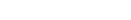
\includegraphics{ch04/figs/resistor-symbol}}
and in the description of the circuit of which the box is one component,
we replace the box with this abstraction. An electrical circuit or
network is then a collection of such circuit elements joined to one
another by paths of negligible resistance.

Taking a network consisting of many elements connected together
and selecting two points as terminals, we can regard the whole thing
as equivalent, as far as these two terminals are concerned, to a single
resistor. We say that the physical network of objects in Fig. 4.9a is
represented by the diagram of Fig. 4.9b and for the terminals $A_1A_2$
% p. 131
the equivalent circuit is Fig. 4.9c. The equivalent circuit for the terminals
at $B_1B_2$ is given in Fig. 4.9d. If you put this assembly in a
box with only that pair of terminals accessible, it will be indistinguishable
from a resistor of $57.6\ \ohmunit$ resistance. There is one very
important ru1e---only \emph{direct-current} measurements are allowed! All
that we have said depends on the current and electric fields being
constant in time; if they are not, the behavior of a circuit element
may not depend on its resistance alone. The concept of equivalent
circuit can be extended from these dc networks to systems in which
current and voltage vary with time. Indeed, that is where it is most
valuable. We are not quite ready to explore that domain.

Little time will be spent here on methods for calculating the
equivalent resistance of a network of circuit elements. The cases of
series and parallel groups are easy. A combination like that in
Fig. 4.10 is two resistors, of value $R_1$ and $R_2$, in series. The equivalent
resistance is
\begin{equation}
  R = R_1 + R_2
\end{equation}
% p. 132
A combination like Fig. 4.11 is two resistors in parallel. By an argument
that you should be able to give, the equivalent resistance R is
found as follows:
\begin{equation}
  \frac{1}{R} = \frac{1}{R_1} + \frac{1}{R_2} \qquad \text{or} \qquad
  R = \frac{R_1R_2}{R_1+R_2}
\end{equation}

That is all that is needed to handle a circuit like the one shown in
Fig. 4.12, which for all its ornateness can be reduced, step by step,
to series or parallel combinations. However, the simple network of
Fig. 4.13 \emph{cannot} be so reduced, so a more general method is required.
Any conceivable network of resistors in which a constant current is
flowing has to satisfy these conditions:

\begin{enumerate}[(i)]
\item The current through each element must equal the voltage
across that element divided by the resistance of the
element.

\item At a \emph{node} of the network, a point where three or more connecting
wires meet, the algebraic sum of the currents into
the node must be zero. (This is our old charge-conservation condition, Eq. 7, in circuit language.)

\item The sum of the potential differences taken in order around
a \emph{loop} of the network, a path beginning and ending at the
same node, is zero. (This is network language for the
general property of the static electric field: $\int\vc{E}\cdot\der\vc{s}=0$ for
any closed path.)
\end{enumerate}

The algebraic statement of these conditions for any network will
provide exactly the number of independent linear equations needed
to ensure that there is one and only one solution for the equivalent
resistance between two selected nodes. We assert this without proving
it. It is interesting to note that the structure of a dc network
problem depends only on the \emph{topology} of the network, that is, on
those features of the diagram of connections that are independent
of any distortion of the lines of the diagram.

A dc network of resistances is a linear system---the voltages and
currents are governed by a set of linear equations, the statements of
the conditions (i), (ii), and (iii). Therefore the superposition of
different possible states of the network is also a possible state. 
Figure 4.14 shows a section of a network with certain currents, $I_1$,
$I_2$, \ldots, flowing in the wires and certain potentials, $V_1$, $V_2$, \ldots, at
the nodes. If some other set of currents and potentials, say $I'_1$, \ldots,
% p. 133
$V'_1$, \ldots, is another possible state of aff'airs in this section of network,
then so is the set $(1_1 + I'_1)$, \ldots, $(V_1 + V'_1)$, \ldots. These currents
and voltages corresponding to the superposition will also satisfy the
conditions (i), (ii), and (iii). Certain general theorems about 
networks, interesting and useful to the electrical engineer, are based
on this.

\section{Energy dissipation in current flow}

The flow of current in a resistor involves the dissipation of energy.
If it takes a force $\vc{F}$ to push a charge carrier along with average
velocity $\vc{v}$, any agency that accomplishes this must do work at the
rate $\vc{F}\cdot\vc{v}$. If an electric field $\vc{E}$ is driving the ion of charge $q$, then
$\vc{F} = q\vc{E}$, and the rate at which work is done is $q\vc{E}\cdot\vc{v}$. The energy
thus expended shows up eventually as heat. In our model of ionic
conduction the way this comes about is quite clear. The ion acquires
some extra kinetic energy, as well as momentum, between collisions.
A collision, or at most a few collisions, redirects its momentum at
random but does not necessarily restore the kinetic energy to normal.
% p. 134
For that to happen the ion has to transfer kinetic energy to the obstacle
that deflects it. Suppose the charge carrier has a considerably
smaller mass than the neutral atom it collides with. The average
transfer of kinetic energy is small when a billiard ball collides with
a bowling ball. Therefore the ion (billiard ball) will continue to
accumulate extra energy until its average kinetic energy is so high
that its average loss of energy in a collision equals the amount gained
between collisions. In this way, by first ``heating up'' the charge
carriers themselves, the work done by the electric force driving the
charge carriers is eventually passed on to the rest of the medium as
random kinetic energy, or heat.

Suppose a steady current $I$, in amperes, flows through a resistor
of $R$ ohms. In every second, $I$ coulombs of charge are transferred
through a potential difference of $V$ volts, where $V = IR$. Hence the
work done in 1 sec is $I^2R$, in joules. (1 coulomb $\times$ 1 volt = 1 joule =
$10^7$ ergs.) The watt, or volt-ampere, is the corresponding unit of
power $P$ (rate of doing work). (1 watt = 1 joule/sec.)
\begin{equation}
  P = I^2 R
\end{equation}

Naturally the steady flow of current in a dc circuit requires some
source of energy capable of maintaining the electric field that drives
the charge carriers. Until now we have avoided the question of the
\intro{electromotive force} by studying only parts of entire circuits; we kept
the ``battery'' out of the picture. In Sec. 4.10 we shall discuss some
sources of electromotive force.

\section{Electromotive force and the voltaic cell}

The origin of the electromotive force in a direct-current circuit is
some mechanism that transports charge carriers in a direction opposite
to that in which the electric field is trying to move them.
A Van de Graaff electrostatic generator\index{Van de Graaff generator} (Fig. 4.15) is an example on
a large scale. With everything running steadily, we find current in
the external resistance flowing in the direction of the electric field $\vc{E}$,
and energy being dissipated there (appearing as heat) at the rate
$I V_0$, or $I^2R$. Inside the column of the machine, too, there is a 
downward-directed electric field. Here charge carriers can be moved
against the field if they are stuck to a nonconducting belt. They are
stuck so tightly that they can't slide backward along the belt in the
generally downward electric field. (They can still be removed from
the belt by a much stronger field localized at the brush in the 
% p. 135
terminal. We need not consider here the means for putting charge on and
off the belt near the pulleys.) The energy needed to pull the belt is
supplied from elsewhere---usually by an electric motor connected to
a power line, but it could be a gasoline engine, or even a man turning
a crank. This Van de Graaff generator is in effect a battery with an
electromotive force, under these conditions, of $V_0$ volts.

In ordinary batteries it is chemical energy that makes the charge
carriers move through a region where the electric field opposes their
motion. That is, a \emph{positive} charge carrier may move to a place of
higher electric potential if by so doing it can engage in a chemical
reaction that will yield more energy than it costs to climb the electrical
hill.

To see how this works, let us examine one particular voltaic cell.
\intro{Voltaic cell} is the generic name for a chemical source of electromotive
force. In the experiments of Galvani around 1790 the famous
twitching frogs' legs had signaled the chemical production of electric
current. It was Volta who proved that the source was not ``animal
electricity,'' as Galvani maintained, but the contact of dissimilar
metals in the circuit. Volta went on to construct the first battery, a
stack of elementary cells, each of which consisted of a zinc disk and
a copper disk separated by moistened pasteboard. Volta's ``pile,'' as
it was called, was the first practical source of steady electric current.
There are many kinds of voltaic cells, including the ubiquitous ``dry
cell.'' The automobile battery consists, if it is a ``12-volt'' battery, of
six lead-sulfuric acid cells in series. We shall describe another
variety of cell, the \intro{Weston standard cell}, the chemistry of which
happens to be rather simple. In addition, the Weston cell is uniquely
important in the laboratory as the standard for precise voltage
measurements.

One form of Weston cell is illustrated in Fig. 4.16. The device
consists of an H-shaped glass container filled with an aqueous solution
of cadmium sulfate, $\zu{CdSO}_4$. An external lead is sealed into the
bottom of each leg, making contact to the inner electrodes. These
consist, on the left, of a pool of pure mercury and, on the right, of a
pool of mercury in which cadmium metal has been dissolved.
(Many metals will dissolve in mercury; such a solution is called an
amalgam.) Above the mercury pool on the left are some crystals of
mercurous sulfate, $\zu{Hg}_2\zu{SO}_4$, a compound that is only very slightly
soluble in water. We find a difference of potential between the external
leads, the one on the left being positive with respect to the one
on the right. (The absolute value of the potential is irrelevant; only
differences are significant here.) What has happened is that some
% p. 136
cadmium ions have gone into the water solution from the amalgam,
each leaving two electrons behind, until the amalgam electrode is
left with a substantial negative charge. This exodus stopped, how-
ever, when the electrode contained so many extra electrons that their
attraction discouraged any more cadmiums from abandoning their
electrons and leaving.

If we now provide an external conduction path by connecting a
resistor across the cell, electrons will flow over this external path
from the negative electrode to the positive electrode. This will allow
more Cd'' ions to go into solution, the electrons they leave behind
merely replenishing the negative charge on that electrode. A steady
current will continue, accompanied by a migration of ions, completing
the circuit, through the aqueous solution. Meanwhile, things
are happening at the other electrode. Figure 4.17 shows what is
going on, while current is flowing around the circuit, at each of the
two interfaces between electrode and solution (electrolyte). In
Fig. 4.17a mercury ions, $\zu{Hg}^+$, are leaving the solution, meeting electrons
coming from the outside, and thus becoming neutral mercury
atoms. They are replaced in the solution by dissolving $\zu{Hg}_2\zu{SO}_4$,
which contributes at the same time a new sulfate ion to the electrolyte.
In Fig. 4.17b cadmium atoms continue to break up, entering
the electrolyte as $\zu{Cd}^{++}$ ions.

The overall effect is essentially the removal of electrons from cadmium
atoms and the addition of electrons to mercury ions. The
chemist would say that cadmium is being oxidized and mercury is
being reduced. The cell runs because this exchange is energetically
preferred. The relative binding of electrons in the structure of the
cadmium atom and in the structure of the mercury atom is such that,
so to speak, mercury ions like to gain electrons more than cadmium
atoms hate to lose them.

Notice that at each interface ions move against the electric field.
It is these transition layers, no more than some tenths of a nanometer thick, that
correspond to the belt in the Van de Graaff generator.

Consider now the electrical potential changes over the whole 
system, both with and without current flowing. In Fig. 4.18 the variation
% p. 137
of potential around the circuit, which is open at one point, is
plotted on a vertical scale. The open-circuit potential difference
between the terminals is the electromotive force of the cell, denoted
by $\emf$. The electric field is the negative gradient of the potential. As
in any other electrostatic field, the line integral of $\vc{E}$ around the 
complete path is zero. (By the way, the level at which the potential of
the electrolyte has been drawn is rather arbitrary---one cannot
directly measure it.)

Figure 4.19 shows the potential distribution when current is 
flowing through an external resistor. Within the electrolyte there is an
electric field in the direction of current flow. The cadmium sulfate
solution acts like an ordinary ohmic resistance. The potential difference
at the terminals is now less than $\emf$, owing to the internal potential
drop across the electrolyte, and possibly also to extra resistance
in the transition layers. The line integral of the electric field
around the whole circuit is still zero. If current flows until $Q$ coulombs
of charge have passed any point in the circuit, then $\emf Q$, with
$\emf$ in volts, is the energy in joules that has been dissipated, externally
and internally, at the expense of the chemical energy of the cell
constituents.

The chain of reactions in the cell is reversible. That is, if another
source, of greater electromotive force, were connected into the circuit
in opposition, current would flow the other way and the processes
we have described would run backward. That's what happens when
a storage battery is charged. In the common ``dry cell,'' some
irreversible changes occur during discharge, precluding reversal of
the process.

The electromotive force of a cell depends on atomic properties.
The values lie in the range of a volt or so because the binding energies
of the outer electrons of atoms are in the range of several electron
volts, and it is essentially the differences in these binding energies
% p. 138
that are manifest in the electromotive force. The electromotive force
depends somewhat on the temperature, a reminder that the proper
treatment of electrochemical processes is a problem in 
thermodynamics. It is a central topic in physical chemistry. Strictly speaking,
it is not the energy, but the so-called \emph{free energy}\index{free energy} that is involved,
a thermodynamic distinction we cannot go into here.

The Weston cell itself is not used as a source of electrical energy but
rather as a standard for potential difference. The situation depicted
in Fig. 4.19, in which so large a current is flowing that the terminal
voltage has dropped by about 10 percent, would be a gross misuse of
the cell. The electromotive force of the Weston cell is highly 
reproducible. In a slightly different version, in which the aqueous solution
is saturated with excess cadmium sulfate near both electrodes, the
electromotive force at $20\degcunit$ is 1.0183 volts. Using a Weston cell as
a standard and a suitable potentiometer, voltages can be reliably
measured to an accuracy of one part in 100,000.

So far as its role in an external circuit is concerned, a cell can be
well represented by an equivalent circuit consisting of an electromotive
force $\emf$ in series with a certain internal resistance $R_i$. 
Connection to an external resistance $R$ results in a current
\begin{equation*}
  I = \frac{\emf}{R+R_i}
\end{equation*}
as shown in Fig. 4.20.

\section{Variable currents in capacitors and resistors}

Let a capacitor of capacitance $C$ be charged to some potential $V_0$
and then discharged by suddenly connecting it across a resistance $R$.
Figure 4.21 shows the capacitor indicated by the conventional
symbol
\raisebox{-0.1\height}{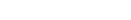
\includegraphics{ch04/figs/capacitor-symbol}},
the resistor $R$, and a switch which we shall imagine to
be closed at time $t = 0$. It is obvious that as current flows the
capacitor will gradually lose its charge, the voltage across the capacitor
will diminish, and this in turn will lessen the flow of current. To
see exactly what happens we need only write down the conditions
that govern the circuit. Let $Q$ be the charge on the capacitor at any
instant, $V$ the potential difference between the plates which is also
the voltage across the resistance $R$. Let $I$ be the current, considered
positive if it flows away from the positive side of the capacitor. These
quantities, all functions of the time, must be related as follows:
\begin{equation}
  Q = CV \qquad I=\frac{V}{R} \qquad -\frac{\der Q}{\der t} = I
\end{equation}
% p. 139
Eliminating $I$ and $V$, we obtain the equation which governs the time
variation of $Q$:
\begin{equation}
  \frac{\der Q}{\der t} = -\frac{Q}{RC}
\end{equation}
Writing this in the form
\begin{equation}
  \frac{\der Q}{Q} = -\frac{\der t}{RC}
\end{equation}
we can integrate both sides, obtaining
\begin{equation}
  \ln Q = -\frac{-t}{RC} + \text{const}
\end{equation}
The solution of our differential equation is therefore:
\begin{equation}
  Q = (\text{another constant}) \times e^{-t/RC}
\end{equation}

We said that at $t = O$, $V = V_0$, so that $Q = CV_0$ for $t = O$. This
determines the constant and we now have the exact behavior of $Q$
after the switch is closed:
\begin{equation}
  Q = CV_0 e^{-t/RC}
\end{equation}
The behavior of the current $I$ is found directly from this:
\begin{equation}
  I = -\frac{\der Q}{\der t} = \frac{V_0}{R} e^{-t/RC}
\end{equation}

At the closing of the switch the current rises at once to the value
$V_0/R$ and then ``decays'' exponentially to zero. The time that characterizes
this decay is the constant $RC$. We should not be surprised to
find that the product of resistance and capacitance has the dimensions
of time, for we know that $C$ has the dimensions of length, and
we have already remarked that \emph{resistance} $\times$ \emph{length}, when it appears
as $\ohmunit\unitdot\cmunit$, the unit of resistivity, has the dimensions of time. People
often speak of the ``$RC$ time constant'' associated with a circuit or
part of a circuit.

In the practical system of units the unit of capacitance is the \intro{farad}.
A capacitor of one farad capacitance has a charge of one coulomb
for a potential difference of one volt. With $R$ in ohms and $C$ in
farads, the product $RC$ is a time in seconds. Just to check this,
note that ohm = volt/ampere = $\zu{volt}\unitdot\sunit/\zu{coulomb}$, while farad =
coulomb/volt. If we make the circuit of Fig. 4.21 out of a 0.05-microfarad
% p. 140
capacitor and a $5\ \zu{M}\ohmunit$ resistor, both of which are
reasonable objects to find around any laboratory, we would have
$RC = 5 \times 10^6 \times 0.05 \times 10^{-6}$ or 0.25 s.

Quite generally, in any electrical system made up of charged conductors
and resistive current paths, one time scale---perhaps not the
only one---for processes in the system is set by some resistance-
capacitance product. This has a bearing on our earlier observation
about the dimensions of resistivity. Imagine a capacitor with plates
of area $A$ and separation $s$. Its capacitance $C$ is $A/(4\pi s)$. Now
imagine the space between the plates suddenly filled with a conductive
medium of resistivity $\rho$. To avoid any question of how this might
affect the capacitance, let us suppose that the medium is a very
slightly ionized gas; a substance of that density will hardly affect the
capacitance at all. This new conductive path will discharge the
capacitor as effectively as did the external resistor in Fig. 4.21. How
quickly will this happen? The resistance of the path, $R$, is $\rho s/A$.
Hence the time constant $RC$ is just $(\rho s/A)(A/4\pi s) = \rho/4\pi$. This
time is independent of the proportions and the absolute size of the
capacitor. What we have here is simply the time constant for the
process of redistribution of charge or relaxation of the electric field,
in a conducting medium. We really didn't need the capacitor plates
at all to describe the situation. If we place two sheets of charge opposite
one another in a conducting medium, they will presently dis-
appear, the electric field will vanish, and the medium will be restored
to a constant potential. The \intro{relaxation time} is determined by the
resistivity $\rho$. For instance, if our weakly ionized gas had a resistivity
of $10^3\ \ohmunit\unitdot\cmunit$, the relaxation time ought to be about $10\ \mu\sunit$.

We remember that really good conductors like the metals have
resistivities of the order of $10^{-5}\ \ohmunit\unitdot\cmunit$, which we now see implies
a relaxation time of the order of $10^{-18}\ \sunit$. A number like this should
arouse our suspicion. Can it really be interpreted as the time required
for dissipation of a charge concentration in a conductor? We
note first of all that it is much shorter than any collision time or correlation
time that we might infer from our model of electrical con-
ductivity. In Eq. 19 we found $\tau_- = 3\times 10^{-14}\ \sunit$ for sodium at
room temperature. This already warns us that for phenomena on
so short a time scale we have no right whatever to use the ``dc'' resistivity
$\rho$. This throws doubt on any quantitative estimate of a
relaxation time.

However there is an even deeper reason to suspect that the story
is not complete. That is the curious fact that our electrical relaxation
% p. 141
time $T = \rho/4\pi$ appears to be independent of the size of the region
involved. That is all very well if the region is small enough, but for
any finite relaxation time $T$, if the region involved has one dimension
greater than $T$ times the speed of light, the relaxation would involve
the propagation of a charge readjustment at a speed greater than $c$.
That would be incompatible with relativity. Thus we see already
that if the behavior of electric charges and fields is to be consistent
with the postulates of special relativity, something more has to come
into the picture. That will be the subject of our next chapters.
